
In questo capitolo vengono presentati i risultati ottenuti dall'algoritmo CUTE. 
In primo luogo sono analizzati i dataset utilizzati nei test svolti.
Successivamente sono mostrati i risultati ottenuti da CUTE per quanto riguarda i cluster individuati e le performance in relazione al tempo.
Infine è discusso il confronto tra CUTE e SPARE: sono presentate le differenze tra gli approcci e i risultati ottenuti.

I test sono stati eseguiti su un cluster composto da 15 nodi, ognuno dei quali equipaggiato con un 8-core i7 CPU 3.60Hz e 32GB di RAM e interconnessi da una ethernet Gigabit.


\section{Dataset}\label{sec:comp:dataset}
Nel processo di testing e confronto tra i due algoritmi sono stati impiegati due diversi dataset.

Il primo dataset utilizzato è Geolife (\cite{GeolifeG31:online}).
Questo dataset è composto da un insieme di traiettorie raccolte in Asia, in particolare in prossimità della città di Pechino.
In Geolife sono presenti 17158 traiettorie distinte, composte da punti contenenti latitudine, longitudine e altitudine.
Il \(91\%\) delle traiettorie nel dataset sono generate da dispositivi aventi tempo di campionamento compreso tra \(1\) e \(5\) secondi.
Il tempo totale coperto da tutte le traiettorie nel dataset è circa quattro anni.

Il secondo dataset impiegato è composto da un insieme di traiettorie registrate nella città di Oldenburg.
Questo conta 1000000 traiettorie, a differenza di quanto detto prima, i punti non sono espressi in coordinate polari, ma in coordinate cartesiane rispetto a un sistema di riferimento custom.
Anche per quanto riguarda la dimensione temporale, il dataset viene fornito con punti aventi una componente temporale relativa a una sequenza di istanti.
La sequenza in questione conta 245 istanti distinti.

La \cref{tab:metrics-dataset} riassume le caratteristiche principali dei dataset impiegati nei test.
Per quanto riguarda il numero di traiettorie, Geolife viene utilizzato sempre nella sua interezza, Oldenburg invece partizionato diversamente a seconda delle situazioni di impiego.


\begin{table}[H]
    \centering
   \begin{tabular}{||c c c c c||}
 \hline
     Dataset & Spazio & Tempo & Punti & Traiettorie\\ [0.4ex] 
 \hline\hline
    Geolife & Coordinate polari & yyyy-mm-gg hh:mm:ss & 18891115 & 17158 \\ 
 \hline
     Oldenburg & Coordinate cartesiane & Sequenziale & 64895840 & 1000000 \\ 
 \hline
\end{tabular}
    \caption{Riassunto delle caratteristiche principali dei due dataset utilizzati}
    \label{tab:metrics-dataset}
\end{table}


\section{CUTE}\label{sec:comp:cute}
Di seguito sono presentati tutti i test eseguiti su CUTE.
Questi test sono stati condotti, salvo specificato diversamente, su un insieme di \(9\) executors, aventi ciascuno \(3\) cores.
Ad ogni executor sono stati assegnati \(12\) gigabyte di RAM.

\subsection{Cluster individuati}\label{subsec:comp:cluster}
Scopo dell'algoritmo CUTE è la ricerca di pattern di movimento aventi caratteristiche di rilevanza rispetto al percorso e dimensione del gruppo in movimento.
Essendo CUTE un framework generico, deve essere possibile distinguere le varie tipologie di pattern di movimento (swarm, flock, platoon) e verificare le variazioni nel numero degli itemset.
Intuitivamente, una ricerca di swarm produrrà molti più itemset validi di una di flock, per via dei vincoli più rilassati.
Allo stesso modo i diversi livelli di grana delle celle dovranno produrre risultati diversi a seconda delle soglie di supporto e dimensioni.
Per condurre questi test, il dataset utilizzato è stato Geolife, in quanto compatibile con le scale settimanale e giornaliera.

Primo e fondamentale ambito di testing è stato il sistema di riferimento e di conseguenza la granularità di ogni cella.
Questo parametro risulta particolarmente interessante: in un algoritmo di row enumeration, come CUTE o Carpenter, il numero di transazioni determina la complessità dell'algoritmo.
Come detto nella \cref{sec:cute:cim}, nel primo passo della ricerca dei gruppi, ogni cella corrisponde a una transazione.
A seconda del valore dei parametri \(s\) e \(t\), ovvero l'intervallo spaziale e quello temporale, il volume di ogni cella e il loro numero complessivo cambia.
Le \cref{fig:chap-4:cells} mostra il numero di celle al variare del lato \(s\) tra \(1,5,10\)KM.
All'aumentare del lato spaziale delle celle, la compressione dello spazio di ricerca aumenta, diminuendo quindi il numero di celle.
La \cref{fig:chap-4:cellt} mostra invece il rapporto tra \(t\) che varia su \(24h,7gg\) e in assenza di dimensione temporale e le celle. 
Com'è possibile vedere, il numero delle celle a parità di spazio non cresce esponenzialmente, ma di un fattore moltiplicativo collegato ai possibili valori dell'intervallo temporale.

\begin{figure}
  \centering
  \begin{subfigure}{.5\textwidth}
  \centering
   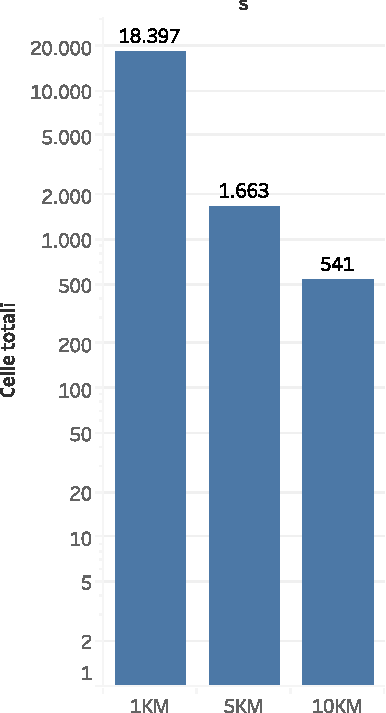
\includegraphics[scale=0.5]{res/fig/sec-4/Cells.pdf}
   \caption{\(s\) tra \(1,5,10\) KM}
  \label{fig:chap-4:cells}
\end{subfigure}%
\begin{subfigure}{.5\textwidth}
  \centering
   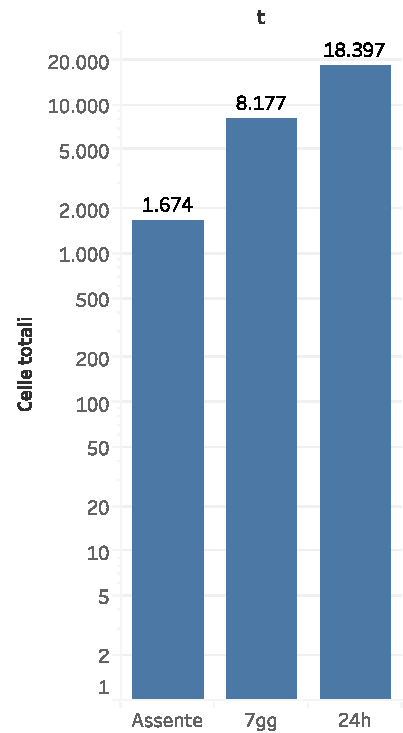
\includegraphics[scale=0.5]{res/fig/sec-4/CellT.pdf}
   \caption{\(t\) tra 24h, 7gg e assenza di tempo}
  \label{fig:chap-4:cellt}
\end{subfigure}%
  \caption{Celle alla variazione di \(s\) a sinistra, \(t\) a destra}%
  \label{fig:chap-4:cellst}
\end{figure}

Su ognuna delle configurazioni sopra espresse è stata eseguita una ricerca di itemset rispetto alle variazioni dei parametri in gioco presentati nella \cref{subsec:cute:params}.
I valori espressi per questi parametri sono riassunti nella \cref{tab:parameters-variation}.
Nei successivi test, dove non specificato, ai parametri è assegnato il valore di default (in grassetto nella \cref{tab:parameters-variation}).

\begin{table}[H]
    \centering
   \begin{tabular}{||c c c||}
 \hline
     Param. & Significato & Valori \\ [0.4ex] 
 \hline\hline
   s & Lato spaziale cella & \textbf{1KM}, 5KM, 10KM \\
   \hline
   t & Lato temporale cella & \textbf{24h}, 7gg, assenza di tempo \\
   \hline
   minsize & dimensione dei gruppi & 5, \textbf{10}, 15 \\
   \hline
   minsup & supporto minimo & 5, \textbf{10}, 15 \\
   \hline
   \(\epsilon\) & soglia spaziale & 2, \textbf{5}, 10, \(\infty\) \\
   \hline
   \(\tau\) & soglia temporale & 1, \textbf{2}, \(\infty\) \\
 \hline
\end{tabular}
    \caption{Parametri e il loro valore di default (in grassetto)}
    \label{tab:parameters-variation}
\end{table}

In particolare il focus di questi test è capire come varia il numero dei cluster individuati all'interno del problema.
I valori di supporto e dimensione minima coincidono e sono stati determinati empiricamente.
Il range di \(\epsilon\) varia tra \((2, 5, 10, \infty)\) mentre quello di \(\tau\) tra \((1, 2, \infty)\).
Mentre i valori di \(\epsilon\) sono stati scelti sperimentalmente, quelli di \(\tau\) sono stati selezionati sulla base del range delle scale temporali utilizzate.
In particolare le scale giornaliere e settimanale presentano una natura ciclica.
Una scala ciclica non ha un valore massimo assoluto e un minimo assoluto, ma prevede che il valore successivo al massimo sia il minimo.
Questa circolarità impatta la misura della distanza tra due punti.
Questa è definita come la dimensione del più piccolo intervallo tra due punti: può essere quindi la minima distanza calcolata dal maggiore al minore o viceversa.
Ciò comporta che all'interno di una scala ciclica, i valori siano molto più vicini rispetto a una monotona.
Quindi è molto facile che considerando valori alti di \(\tau\) il risultato tenda a essere quello di \(\tau = \infty\).
Ciò vale soprattutto per la scala settimanale: essendo solamente \(7\) i giorni della settimana e la scala ciclica per definizione, la distanza massima tra due qualunque elementi è al massimo \(3\).
Questo implica che l'unico valore plausibile per eseguire una ricerca di platoon su questa scala sia \(2\).
\(\tau\) determina inoltre la categoria di co-movement pattern individuato, ad esempio su scala settimanale vale che:
\begin{itemize}
    \item \(\tau = 1\): Flock
    \item \(\tau = 2\): Platoon g-connected
    \item \(\tau = \infty\): Swarm
\end{itemize}

\begin{figure}
  \centering
  \begin{subfigure}{.5\textwidth}
  \centering
   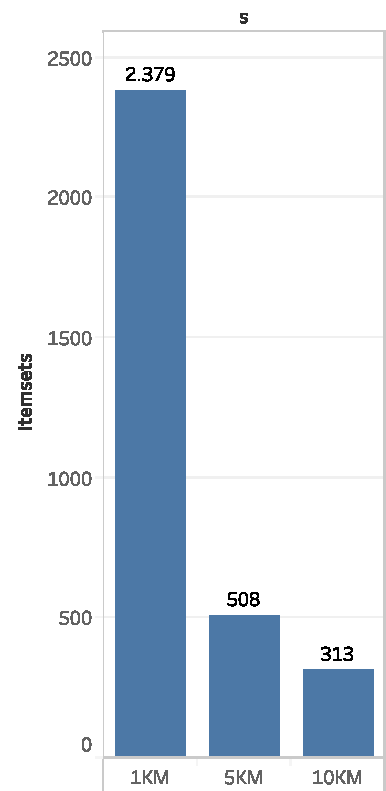
\includegraphics[scale=0.5]{res/fig/sec-4/itemset/ItemsetS.pdf}
   \caption{\(s\) tra \(1,5,10\) KM}
  \label{fig:chap-4:ItemsetS}
\end{subfigure}%
\begin{subfigure}{.5\textwidth}
  \centering
   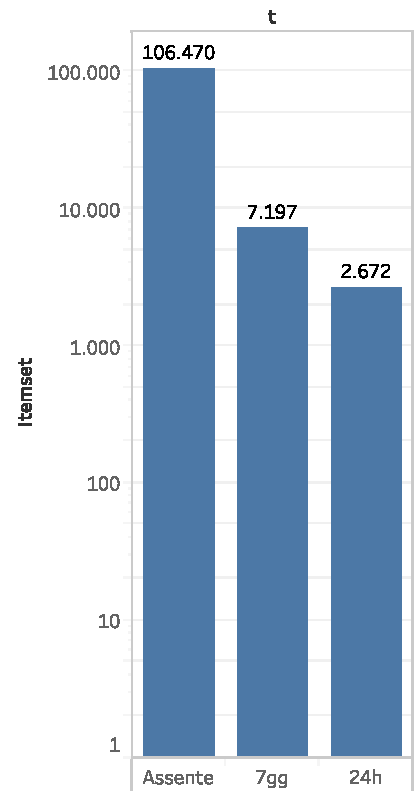
\includegraphics[scale=0.5]{res/fig/sec-4/itemset/ItemsetT.pdf}
   \caption{\(t\) tra 24h, 7gg e assenza di tempo}
  \label{fig:chap-4:ItemsetT}
\end{subfigure}%
  \caption{Numero di itemset alla variazione di \(s\) a sinistra, \(t\) a destra}%
  \label{fig:chap-4:ItemsetSandT}
\end{figure}

Le \cref{fig:chap-4:ItemsetS,fig:chap-4:ItemsetT} mostrano le variazioni del numero di itemset su \(s\) e \(t\).
Per quanto riguarda le variazioni nel lato spaziale delle celle \(s\), i risultati sono coerenti con quanto atteso: all'aumentare dell'area coperta dalle celle, calano il numero di itemset individuati (\cref{fig:chap-4:ItemsetS}).
Ciò è coerente con la natura del problema: se ogni cella corrisponde a una transazione, al calare del numero di transazioni a parità di supporto calano sia il numero di itemset frequenti che il tempo necessario per eseguire la ricerca.
Per \(t\), i risultati presentati sono stati ottenuti ponendo \(\tau = \infty\), questo perché non avrebbe avuto senso considerare la continuità nel tempo considerando una scala come l'assenza di tempo che esclude questa dimensione (\cref{fig:chap-4:ItemsetT}).
Alla luce di ciò, la dimensione temporale \(t\) presenta invece un trend opposto a \(s\) per quanto riguarda gli itemset individuati: l'impiego della scala giornaliera rispetto a quella settimanale individua meno itemset sia in caso di vincoli su \(\tau\) che in sua assenza.
L'assenza di una dimensione temporale invece produce risultati di circa un ordine di grandezza superiori rispetto agli altri due.
Questo fenomeno può essere direttamente collegato all'aumento del numero di celle a seguito dell'adozione di diverse scale temporali.
L'introduzione di una nuova dimensione produce infatti un'ulteriore suddivisione dello spazio di ricerca: un pattern valido in uno spazio \(n\)-dimensionale può non risultarlo più in uno \(n+1\) dimensionale, poiché il gruppo può non risultare vicino nella nuova dimensione.
Questa frammentazione sarà tanto più netta tanti più valori possibili avrà la scala della nuova dimensione.
Applicando quanto detto sopra alle scale temporali, l'assenza di tempo non produce nessuna ulteriore divisione, la scala settimanale e quella temporale aggiungono una cardinalità di rispettivamente \(7\) e \(24\) intervalli.
La frammentazione dello spazio di ricerca causa quindi la differenza nei risultati delle tre scale.


Le \cref{fig:chap-4:ItemsetMinsize,fig:chap-4:ItemsetMinsupp} individuano le variazioni di pattern riconosciuti al variare di supporto e dimensione minima.
Minsup e minsize (\(\alpha, \gamma\)) sono fatti variare tra \(5, 10, 15\).
Entrambi i parametri si comportano come atteso: all'aumentare del valore cala il numero di itemset individuati.
La ricerca di gruppi di dimensioni maggiori o che abbiano un elevato tempo di viaggio riduce il numero di itemset validi.

\begin{figure}
  \centering
   \begin{subfigure}{.5\textwidth}
  \centering
    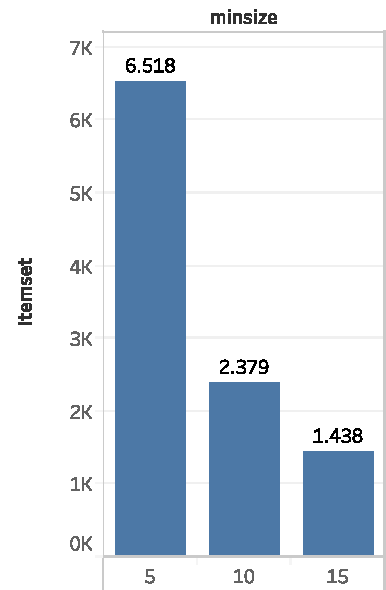
\includegraphics[scale=0.5]{res/fig/sec-4/itemset/ItemsetMinsize.pdf}
   \caption{\(minsize\) tra \(5,10,15\)}
  \label{fig:chap-4:ItemsetMinsize}
\end{subfigure}%
\begin{subfigure}{.5\textwidth}
  \centering
   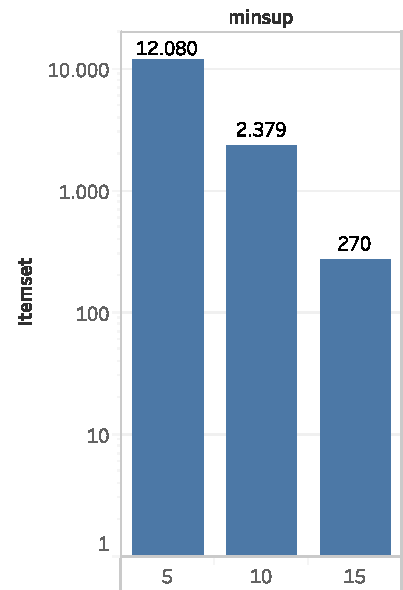
\includegraphics[scale=0.5]{res/fig/sec-4/itemset/ItemsetMinsupp.pdf}
   \caption{\(minsup\)  tra \(5,10,15\)}%
  \label{fig:chap-4:ItemsetMinsupp}
  \end{subfigure}%
  \caption{Numero di itemset alla variazione di \(minsize\) a sinistra e \(minsupp\) a destra}%
  \label{fig:chap-4:ItemsetMinsizeandMinsupp}
\end{figure}

Infine i test condotti su \(\epsilon\) e \(\tau\) mostrano il diverso numero di pattern individuati stringendo o rilassando i vincoli di contiguità.
Per quanto riguarda \(\epsilon\), la \cref{fig:chap-4:ItemsetEpsilon} mostra come il numero di pattern individuati cali al diminuire del valore di soglia.
Questa tendenza rallenta solo nel caso dei valori \(10\) e \(\infty\) dove i risultati quasi coincidono.
I risultati ottenuti su questo parametro sono coerenti con quanto atteso: vincoli più stretti producono meno itemset.
La coincidenza tra il valore \(10\) e \(\infty\) può essere motivata dall'ampiezza del raggio di vicinanza coperto rispetto all'area complessiva del problema.
Un raggio di vicinato pari a \(10\)KM include probabilmente la maggior parte delle celle individuate nello spazio, di conseguenza i suoi risultati tendono a quelli ottenuti rilassando il vincolo.

Per quanto riguarda \(\tau\), è possibile riscontrare come la ricerca di flock, platoon e convoy non produca le differenze attese nei risultati.
Su Geolife le differenze riguardano solo poche tuple tra le tre ricerche.
Questi risultati sono mostrati nella \cref{fig:chap-4:ItemsetTau}.
Questo comportamento è a prima vista inusuale: i vincoli sullo spazio si dimostrano efficaci nella riduzione dello spazio di ricerca mentre quelli sul tempo sono praticamente trascurabili.
Tuttavia occorre considerare la diversità fra la scala spaziale e quella temporale in termini di possibili elementi: quest'ultima infatti ha un range decisamente inferiore rispetto a qualunque scala temporale utilizzata nel corso dei test.
Nel caso di scala giornaliera ad esempio i valori possibili sono \(24\), mentre per quella settimanale sono \(7\).
Come detto nella presentazione di Geolife, i singoli punti hanno frequenze di campionamento molto più elevate della granularità temporale del sistema di riferimento.
Quindi sono poche le traiettorie che hanno una continuità rispetto alle ore del giorno, ancora meno rispetto ai giorni della settimana.

\begin{figure}
  \centering
   \begin{subfigure}{.5\textwidth}
  \centering
    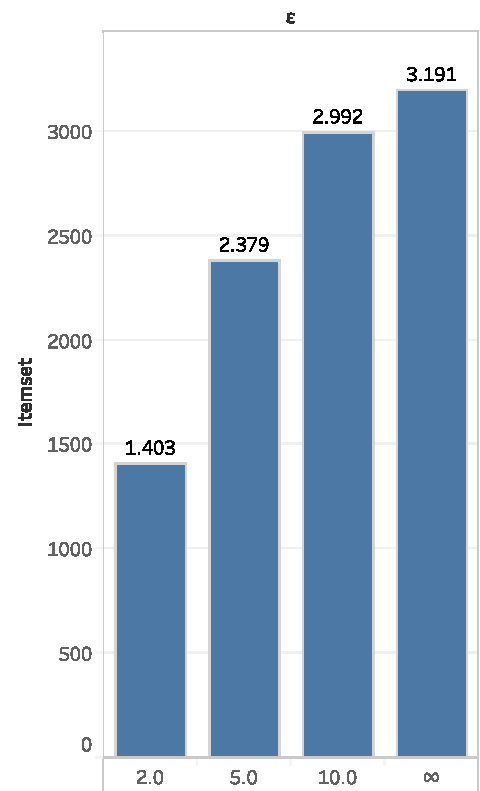
\includegraphics[scale=0.5]{res/fig/sec-4/itemset/ItemsetEpsilon.pdf}
   \caption{\(\epsilon\) tra \(2,5,10,\infty\)}
  \label{fig:chap-4:ItemsetEpsilon}
\end{subfigure}%
\begin{subfigure}{.5\textwidth}
  \centering
   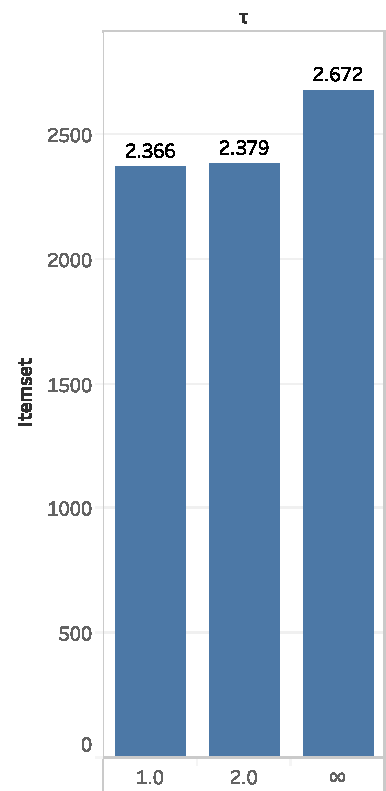
\includegraphics[scale=0.5]{res/fig/sec-4/itemset/ItemesetTau.pdf}
   \caption{\(\tau\) tra \(1,2,\infty\)}%
  \label{fig:chap-4:ItemsetTau}
  \end{subfigure}%
  \caption{Numero di itemset alla variazione di \(\epsilon\) a sinistra e \(\tau\) a destra}%
  \label{fig:chap-4:ItemsetEpsilonAndTau}
\end{figure}




\subsection{Performance}\label{subsec:comp:performance}
In parallelo sono state verificate le performance di CUTE valutando diverse situazioni.
In primo luogo, è stato valutato il tempo di esecuzione rispetto alle configurazioni già presentate nella \cref{subsec:comp:cluster}.
Successivamente sono stati eseguiti test per valutare le tempistiche al variare del numero di risorse fisiche impiegate, ovvero executor e core.
In tutti i test il tempo è sempre registrato in millisecondi.

Nel cronometrare la durata dell'algoritmo, non è considerata la fase di creazione delle tabelle di supporto.
Questo perché le tabelle in questione possono potenzialmente essere create separatamente da CUTE e poi utilizzate dall'algoritmo.
Inoltre a parità di parametri \(s\) e \(t\) una stessa tabella può essere utilizzata da più esecuzioni dell'algoritmo.

Partendo dalle valutazioni basate sull'alterazione dei parametri dell'algoritmo, la \cref{fig:chap-4:TimeSandT} mostrano il tempo di calcolo rispetto alle variazioni dei lati spazio-temporali della cella.
Al crescere di \(s\) (\cref{fig:chap-4:TimeS}), cala il tempo di esecuzione.
Intuitivamente ciò è collegato al numero di celle: celle più grandi e meno numerose corrispondono a meno transazioni da valutare durante la ricerca.
Per \(t\) (\cref{fig:chap-4:TimeT}) la situazione è diversa.
Il trend è inversamente proporzionale al numero di celle: al calare di queste, aumentano i tempi di esecuzione.
Nonostante quindi il numero di celle sia maggiore all'inizio con \(t=24h\), la minor lunghezza delle transazioni porta a generare un minor numero di gruppi da esplorare (come evidenziato anche negli itemset individuati) e causa quindi una diminuzione nei tempi di esecuzione.

\begin{figure}
  \centering
  \begin{subfigure}{.5\textwidth}
  \centering
   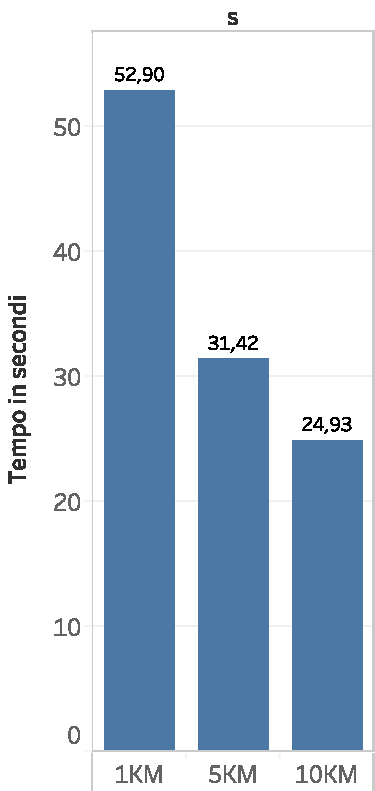
\includegraphics[scale=0.5]{res/fig/sec-4/performance/TimeS.pdf}
   \caption{\(s\) tra \(1,5,10\) KM}
  \label{fig:chap-4:TimeS}
\end{subfigure}%
\begin{subfigure}{.5\textwidth}
  \centering
   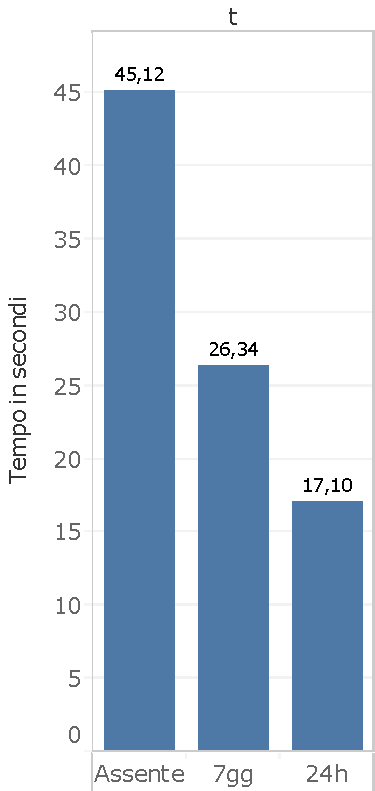
\includegraphics[scale=0.5]{res/fig/sec-4/performance/TimeT.pdf}
   \caption{\(t\) tra 24h, 7gg e assenza di tempo}
  \label{fig:chap-4:TimeT}
\end{subfigure}%
  \caption{Tempo di computazione alla variazione di \(s\) a sinistra, \(t\) a destra}%
  \label{fig:chap-4:TimeSandT}
\end{figure}

Variando \(minsize\) (\cref{fig:chap-4:TimeMinsize}) è possibile vedere un trend di diminuzione dei tempi di esecuzione al crescere del parametro.
Questo è coerente con quanto atteso: la ricerca di gruppi più numerosi comporta il pruning dei piccoli gruppi e risparmia tempo sul tempo di esecuzione globale.
Considerando invece \(minsup\) (\cref{fig:chap-4:TimeMinsupp}), vale lo stesso discorso.
Le ragioni sono analoghe a quanto detto per \(minsize\).


\begin{figure}
  \centering
   \begin{subfigure}{.5\textwidth}
  \centering
    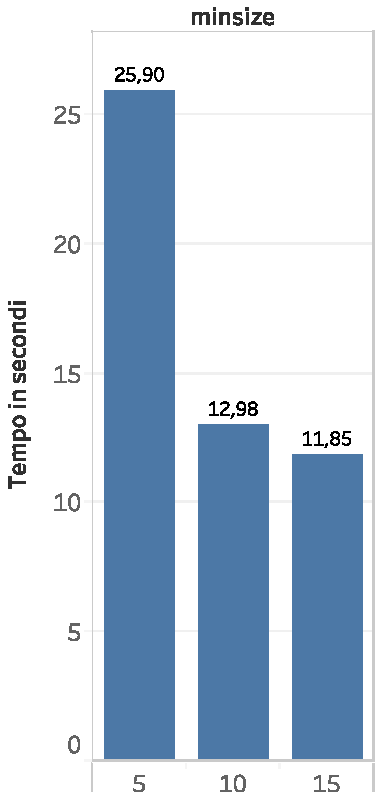
\includegraphics[scale=0.5]{res/fig/sec-4/performance/TimeMinsize.pdf}
   \caption{\(minsize\) tra \(5,10,15\)}
  \label{fig:chap-4:TimeMinsize}
\end{subfigure}%
\begin{subfigure}{.5\textwidth}
  \centering
   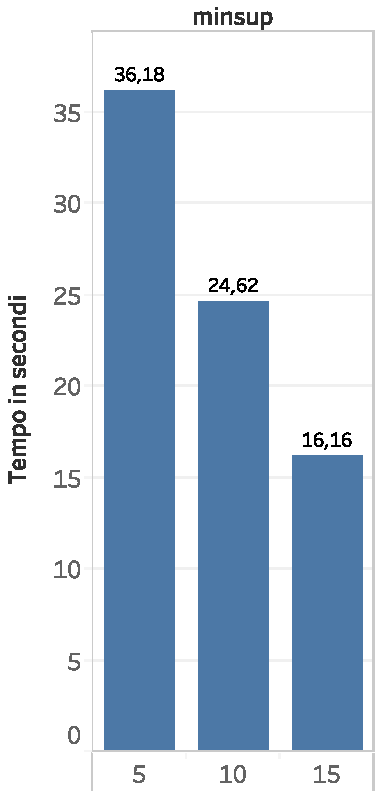
\includegraphics[scale=0.5]{res/fig/sec-4/performance/TimeMisupp.pdf}
   \caption{\(minsup\) tra \(5,10,15\)}%
  \label{fig:chap-4:TimeMinsupp}
  \end{subfigure}%
  \caption{Tempo di computazione alla variazione di \(minsize\) a sinistra e \(minsupp\) a destra}%
  \label{fig:chap-4:TimeMinsizeandMinsupp}
\end{figure}

Trattando poi dei parametri di continuità che riducono lo spazio di ricerca, \(\epsilon\) (\cref{fig:chap-4:TimeEpsilon}) presenta per entrambi i dataset una certa regolarità: al crescere del suo valore, aumenta il tempo di computazione.
Questa regolarità dipende dalla riduzione dello spazio di ricerca effettuato dai vincoli.
Valori più rigidi comportano una maggior riduzione dello spazio di ricerca, che si traduce in un pruning più forte

Su \(\tau\) (\cref{fig:chap-4:TimeTau}) la situazione è più eterogenea: non è possibile individuare un trend definito.
Ancora una volta le cause sono da ricercare nel debole pruning di \(\tau\), la presenza di questo vincolo infatti può in ceri casi rallentare l'esecuzione, in quanto giunge a risultati assimilabili a quelli ottenuti rilassando il vincolo.
Questa ricerca avviene in maniera più lenta, per via delle operazioni aggiuntive sul controllo della continuità.

\begin{figure}
  \centering
   \begin{subfigure}{.5\textwidth}
  \centering
    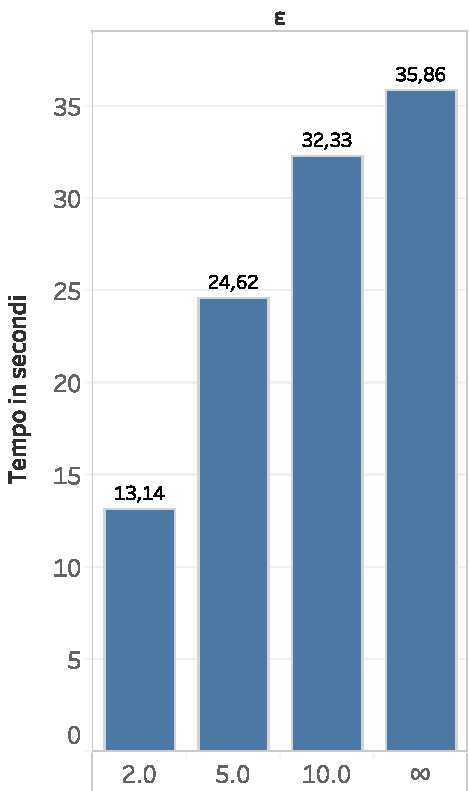
\includegraphics[scale=0.5]{res/fig/sec-4/performance/TimeEpsilon.pdf}
   \caption{\(\epsilon\) tra \(2,5,10,\infty\)}
  \label{fig:chap-4:TimeEpsilon}
\end{subfigure}%
\begin{subfigure}{.5\textwidth}
  \centering
   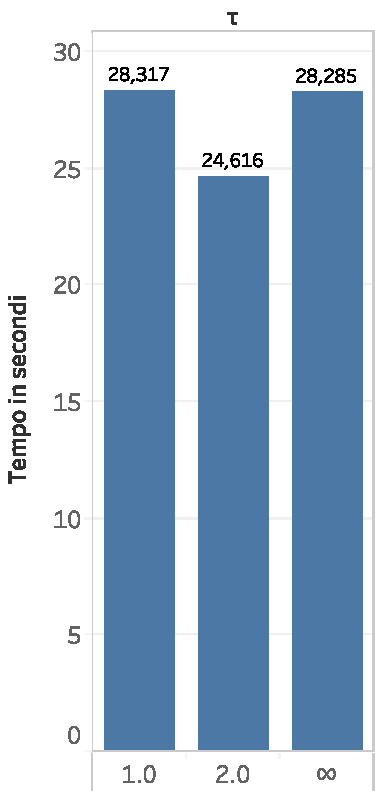
\includegraphics[scale=0.5]{res/fig/sec-4/performance/TimeTau.pdf}
   \caption{\(\tau\) tra \(1,2,\infty\)}%
  \label{fig:chap-4:TimeTau}
  \end{subfigure}%
  \caption{Tempo di computazione alla variazione di \(\epsilon\) a sinistra e \(\tau\) a destra}%
  \label{fig:chap-4:TimeEpsilonAndTau}
\end{figure}

Passando ai test di scalabilità, questi sono stati condotti su un sottoinsieme dei parametri utilizzati nella sezione precedente.
Ciascuna configurazione di parametri è stata testata variando rispettivamente il numero di executor  e quello di core, mantenendo come altri parametri i valori di default specificati nella \cref{tab:parameters-variation}.
La \cref{tab:cores-executors-variation} contiene i valori possibili per core e executor.

\begin{table}[H]
    \centering
   \begin{tabular}{||c c||}
 \hline
     Parametro & Valori \\ [0.4ex] 
 \hline\hline
   core & 2,\textbf{3},4 \\
 \hline
  executor & 5,\textbf{7},9 \\
 \hline
\end{tabular}
    \caption{Valori per core e executor (default in grassetto)}
    \label{tab:cores-executors-variation}
\end{table}


Le \cref{fig:chap-4:ScalabilityCORES,fig:chap-4:ScalabilityEXECUTORS}
mostrano i tempi di esecuzione alla variazione di questi parametri.

\begin{figure}
  \centering
   \begin{subfigure}{.5\textwidth}
  \centering
      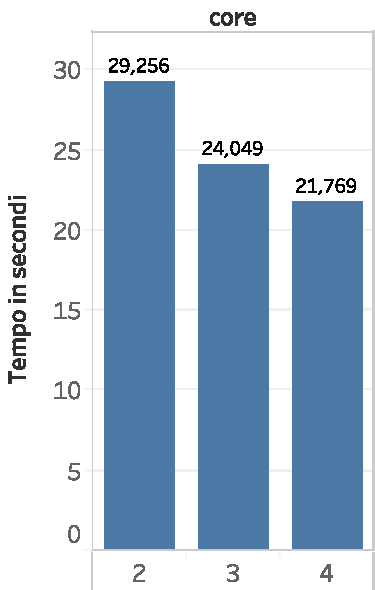
\includegraphics[scale=0.5]{res/fig/sec-4/scalability/ScalabilityDataCORES.pdf}
  \caption{core tra \(2,3,4\)}%
  \label{fig:chap-4:ScalabilityCORES}
\end{subfigure}%
\begin{subfigure}{.5\textwidth}
  \centering
   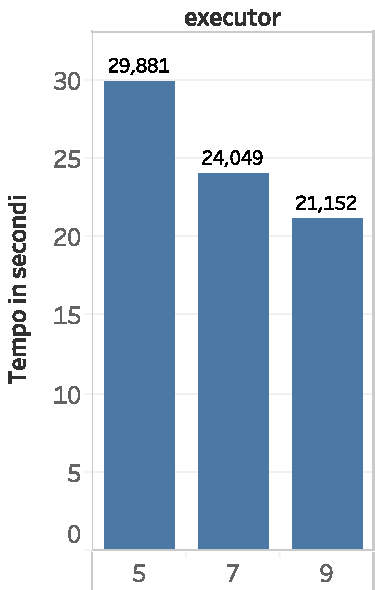
\includegraphics[scale=0.5]{res/fig/sec-4/scalability/ScalabilityDataEXECUTORS.pdf}
  \caption{executor tra \(5,7,9\)}%
  \label{fig:chap-4:ScalabilityEXECUTORS}
  \end{subfigure}%
  \caption{Tempo di computazione alla variazione di core a sinistra e executor a destra}%
  \label{fig:chap-4:ScalabilityCORESandEXECUTORS}
\end{figure}

Com'è possibile notare, la tendenza generale espressa dai grafici è una diminuzione dei tempi di esecuzione all'aumentare dell'impiego di risorse.

Infine per quanto riguarda l'ambito delle performance, sono stati eseguiti alcuni test di scalabilità rispetto al numero di traiettorie.
In particolare per questi è stato utilizzato Oldenburg, in quanto avente un numero di traiettorie molto superiore a Geolife.
La \cref{tab:variation-oldenburg} contiene i parametri di CUTE utilizzati durante queste esecuzioni.

\begin{table}[H]
    \centering
   \begin{tabular}{||c c||}
 \hline
     Parametro & Valore \\ [0.4ex] 
 \hline\hline
 traiettorie & \(50\)K,\(500\)K,\(1.000\)K \\
 \hline
 \(s\) & 1000 \\
 \hline
 \(t\) & 10 \\
 \hline
 \(minsize\) & 100 \\
 \hline
  \(minsupp\) & 10 \\
 \hline
  \(\epsilon\) & \(2\) \\
 \hline
 \(\tau\) & \(1\) \\
 \hline
   core & 3 \\
 \hline
  executor & 9 \\
 \hline
\end{tabular}
    \caption{Valori dei parametri di CUTE utilizzati durante i test sul numero di traiettorie su Oldenburg}
    \label{tab:variation-oldenburg}
\end{table}

I risultati indicano come a parità di risorse, CUTE riesca a gestire in tempi ragionevoli anche un numero di transazioni molto elevato (\cref{fig:chap-4:ScalabilityOldenburg}).
Nel caso peggiore infatti sono necessarie appena 10 minuti per eseguire la ricerca su un milione di traiettorie.
Questo dipende da diversi fattori.
In primo luogo il numero di celle, e di conseguenza quello di transazioni, rimane invariato durante le varie esecuzioni.
Ciò che cambia è quindi la lunghezza media di ogni transazione, che aumenta all'aumentare del numero di traiettorie.
Insiemi di transazioni di diversi ordini di grandezza vengono processati in diversi ordini temporali di grandezza.
Oltre a ciò, questi risultati possono essere collegati a valori molto stringenti per i parametri collegati al pruning, dimostrando così la loro efficacia nel ridurre lo spazio di ricerca.



\begin{figure}
  \centering
  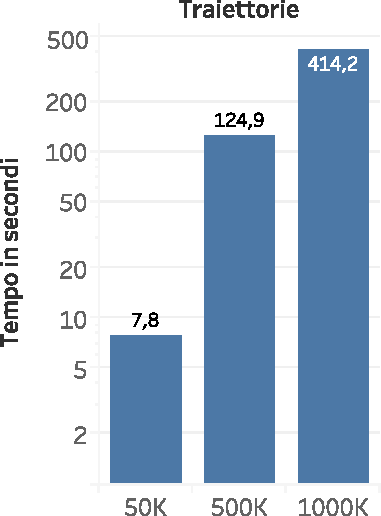
\includegraphics[scale=.5]{res/fig/sec-4/performance/ScalabilityOnOldenburg.pdf}
  \caption{Tempi di esecuzione in secondi variando il numero di traiettorie tra \(50\)K,\(500\)K,\(1000\)K}%
  \label{fig:chap-4:ScalabilityOldenburg}
\end{figure}



\subsection{Considerazioni}\label{subsec:comp:consideration-and-limits}
Alla luce di quanto mostrato riguardo a itemset individuati e performance, si possono trarre le seguenti considerazioni.

In primo luogo i risultati ottenuti confermano l'importanza della suddivisione in quanti sulla base del sistema di riferimento. 
Questo è un aspetto delicato. 
La grana del sistema di riferimento è direttamente collegata con il tipo di pattern che si vuole ricercare.
Differenti ricerche infatti possono portare a differenti suddivisioni dello spazio di ricerca.
Ad esempio una ricerca che consideri la rete stradale di una città avrà sempre molti più quanti di una che considera i quartieri o municipalità di una città.
Occorre quindi valutare il comportamento rispetto alla variazione di transazioni in input e al sistema di riferimento.
Per simulare questo scenario, sono state utilizzate più griglie che hanno permesso di costruire di volta in volta un numero di transazioni arbitrario.

Dai test svolti è emerso che il comportamento dell'algoritmo al variare del numero di celle può essere riassunto come segue:
Per ogni dataset, esiste un sistema di riferimento ideale avente una certa granularità.
Nell'utilizzo di griglie a grana più grossa, a parità di dimensione e supporto minimo, calano le transazioni di esplorare.
Di conseguenza calano gli itemset validi (per via del supporto) e i tempi di esecuzione.
Usando griglie a grana troppo fine, il numero di transazioni aumenta, ma diminuisce la lunghezza di ogni transazione.
In questo caso è la frammentazione a ridurre il numero di elementi in ogni transazione, diminuendo quindi il supporto e la dimensione media degli itemset individuati.
Questo comporta un maggiore pruning e di conseguenza una riduzione nei tempi di calcolo e negli itemset trovati.
In entrambi questi due casi, il sistema di riferimento risulta scarsamente compatibile con le caratteristiche spazio-temporali del dataset.

Per quanto riguarda i parametri di supporto \(minsup\) e dimensione \(minsize\), il comportamento dell'algoritmo è in linea con quanto atteso in ogni situazione.
L'aumentare dei due parametri comporta una riduzione degli itemset validi.
Il pruning di questi itemset diminuisce il volume della ricerca e di conseguenza il costo computazionale totale. 

Altro punto focale emerso dai test è la debolezza nel vincolo di continuità temporale negli itemset individuati: rispetto a quello spaziale infatti il pruning effettuato è molto più debole.
Come già affermato precedentemente, questo dipende dalla finezza della scala impiegata.
Per quanto riguarda la componente spaziale, è improbabile che traiettorie vicine si muovano su celle lontane della mappa.
Per il tempo invece, come affermato nella \cref{subsec:comp:cluster}, le scale delle ore/giorni risultano poco compatibili con l'alto tempo di campionamento delle traiettorie.
Sempre collegato ai vincoli di continuità e alla riduzione dello spazio di ricerca, non sempre accade che una riduzione dello spazio di ricerca comporti un calo nei tempi di esecuzione.
Come affermato nella \cref{subsec:cute:ctm}, il rilassamento dei vincoli sulla continuità nello spazio tempo rende superflue alcune operazione e rende più snella la computazione.
Se quindi il pruning effettuato da questi vincoli è debole, lo spazio di ricerca non sarà ridotto e sarà esplorato più lentamente per via dei vincoli.
Oltre a questo, dal punto di vista implementativo la ricerca di swarm produce meno job da eseguire.
Ogni job spark infatti aggiunge una costo computazionale alla ricerca, in quanto richiede un certo overhead in termini di tempo e risorse per essere creato.

CUTE, come mostrato dai test di scalabilità, ottiene tempi ragionevoli con diverse configurazioni di risorse.
Ciò è possibile grazie al numero contenuto di celle individuate, che risulta sempre molto minore del numero di traiettorie.
Qualora si adottasse una scala temporale assoluta o si riducesse di molto l'area spaziale coperta dalla singola cella, le performance di CUTE calerebbero notevolmente.
La ragione dietro questo calo sarebbe attribuibile all'esplosione del numero di celle.
Con un numero alto di celle, non solo la creazione delle tabelle di supporto aumenta esponenzialmente, ma vengono meno i principi del mining su dataset colossali, in quanto il numero di transazioni (celle) supera quello di item (traiettorie).

\section{CUTE vs SPARE}\label{sec:CUTEvsSPARE}
Terminata l'analisi di CUTE in termini di itemset e tempo di computazione, si passa al confronto tra CUTE e SPARE.
Gli algoritmi approcciano uno stesso problema, la ricerca di pattern di co-movimento, con due tecniche differenti tra di loro.
Questo comporta che durante un confronto, non abbia senso parlare di tempistiche: CUTE e SPARE sono intrinsecamente diversi e la velocità non può essere un buon metro di confronto.
Se il tempo di esecuzione non può essere utilizzato, allora l'intero confronto sarà impostato sulla base dei pattern ottenuti tra i due algoritmi.

\subsection{Confronto tra CUTE e SPARE}\label{subsec:comp:CUTEvsSPARE}
CUTE e SPARE entrambi eseguono una ricerca di pattern di co-movimento.
In tutti e due sono presenti i concetti di lunghezza minima del percorso (\(k, \alpha\)), dimensione minima di un gruppo (\(m, \gamma\)) e massimo gap temporale tra i punti del percorso (\(g, \tau\)).

Parlando poi delle idee di funzionamento dei due algoritmi, in entrambi si utilizzano i concetti di itemset,pruning e monotonicità. 
In CUTE ciò viene realizzato dividendo lo spazio di ricerca in celle, assegnando a ogni cella l'insieme delle traiettorie che transitano nei suoi confini spazio-temporali e eseguendo poi una variante distribuita dell'algoritmo di Carpenter per ricercare cluster di traiettorie.
SPARE invece utilizza un approccio basato su itemset solo nella seconda fase, quella relativa al tempo e formula una propria definizione di monotonicità, diversa dalla frequenza, basata su due parametri \(l\) e \(g\).
Nella prima fase utilizza un clustering spaziale per definire ad ogni istante quali punti sono vicini e quali no.

SPARE prende come ipotesi che per ogni istante della scala temporale, ogni traiettoria abbia al massimo una posizione: questo diventa limitante quando si vuole considerare traiettorie generate da diverse scale di campionamento, poiché l'algoritmo riduce tutte le traiettorie a una scala comune.
Questo processo di semplificazione comporta una perdita di informazioni.

Anche su CUTE è necessario compiere un'operazione di assimilazione a una stessa scala temporale, tuttavia CUTE pone l'enfasi della sua divisione nella creazione di celle con un certo volume nello spazio-tempo.
Dal punto di vista temporale, ogni cella non esprime un istante, ma una durata.
Una traiettoria passa da una cella se transita nei suoi confini anche solo per un istante.
Questo implica che una traiettoria possa muoversi su un range di celle aventi stesso istante temporale.
In questo modo CUTE minimizza la perdita di informazione legata all'adozione di una scala temporale univoca su diverse traiettorie.

Dal punto di vista della vicinanza nello spazio, SPARE è più flessibile sulle forme dei cluster, potendo utilizzare vari algoritmi differenti per la creazione di questi.
Al contrario CUTE ha confini spaziali più rigidi, determinati da una divisione regolare dello spazio.
SPARE però considera la vicinanza solo in termini relativi, trascurando i movimenti eseguiti dal gruppo tra due istanti temporali.
CUTE invece permette di esprimere vincoli sulla contiguità spaziale (\(\epsilon\)) tra le varie celle percorse da un gruppo.

Parlando poi della dimensione temporale, CUTE presenta una gestione omogenea rispetto alla dimensione spaziale, processando quindi spazio e tempo assieme, tuttavia l'algoritmo mostra i suoi limiti in corrispondenza di bucket temporali nell'ordine dei secondi o pochi minuti, a causa dell'aumento del numero di celle. 
SPARE invece ha buone performance anche con bucket temporali nell'ordine dei secondi, inoltre permette una maggiore espressività nei vincoli temporali grazie al vincolo \(l\).
Dall'altro lato però CUTE è in grado di gestire scale temporale cicliche come i giorni della settimana o le ore del giorno, mentre SPARE è limitato a una scala temporale monotona.

CUTE consente inoltre di processare altre dimensioni senza nessuna ulteriore espansione, mentre SPARE è pensato esclusivamente solo per processare dati spazio-temporali.

Trattando infine i risultati, SPARE genera cluster basati su itemset frequenti massimali, CUTE invece su frequenti chiusi. 
CUTE quindi, a parità di configurazione, genererà sempre un numero maggiore di risultati rispetto a SPARE.

\subsection{Risultati a parità di configurazione}\label{subsec:comp:result-comparison}
Come detto nella sezione precedente, CUTE individua itemset chiusi, SPARE massimali.
Per quanto molti passi nei due approcci divergano, è possibile in determinate condizioni ottenere gli stessi risultati tra i due algoritmi.
Ciò però avviene solo in casistiche particolari, nella maggior parte delle situazioni succede che i risultai divergano per alcune caratteristiche intrinseche dei due algoritmi:

\begin{itemize}
    \item \textit{Itemset chiusi \(\supseteq\) Itemset massimali}. È fisiologico, salvo rare eccezioni, che il numero di itemset chiusi in un dataset sia anche di ordini di grandezza più grande di quello dei massimali.
    \item \textit{Le metriche spaziali divergono}.
   L'impiego di due metriche spaziali differenti porta a risultati che in assoluto possono divergere per alcune tuple.
\end{itemize}

Per quanto i due algoritmi possano avere elementi in comune, queste particolarità devono essere tenute in conto durante il confronto dei risultati.
Confrontare il numero di itemset identici produrrebbe quindi scarsi risultati.
Serve perciò definire una metrica di confronto che tenga conto di queste due caratteristiche: non deve penalizzare eccessivamente la differenza nel numero dei risultati e deve misurare la similarità tra gli itemset tenendo conto che questi possono divergere per l'assenza o presenza di qualche elemento.

Alla luce di questo, è stata formulata la seguente misura di similarità \(S\).
Per confrontare i due insiemi di itemset si utilizza una variazione dello Stable Marriage Problem~\cite{mcvitie1971stable}.
Dati due set di stesse dimensioni, questa tecnica permette di assegnare ogni elemento di un set a uno dell'altro sulla base di un criterio di similarità custom.
Questo permette di ottenere una soluzione sub-ottima al problema dell'assegnamento, assicurandosi che non esistano due elementi appartenenti a insiemi diversi che abbiano una similarità maggiore tra di loro rispetto che coi rispettivi partner (\cref{definition:stable-marriage-problem}).

\begin{definition}[Stable Marriage Problem]\label{definition:stable-marriage-problem}

 Dati due insiemi di oggetti \(N\) e \(M\), si definisce problema del matrimonio stabile il problema che ricerca l'insieme delle coppie \((n_i \in N, m_j \in M)\) tali che definita una metrica di similarità \(s\) non esistano in contemporanea due coppie \((n_p, m_p),(n_q,m_q)\) tali che  \(n_p,n_q \in N,m_p,m_q \in M\) per cui vale che: 
  \begin{center}
  \(
    \begin{cases}
     s(n_p,m_j) > s(n_i, m_j) \land s(n_p,m_j) > s(n_p,m_p) \\
     s(n_i, m_q) > s(n_i, m_j) \land s(n_i, m_q) > s(n_q, m_q)
    \end{cases}
    \)
  \end{center}
\end{definition}

Definita la modalità di assegnamento, si rende necessario individuare una metrica di confronto tra i singoli itemset.
Questa è definita via coefficiente di Jaccard.
Questo calcola la similarità tra due set come il numero di elementi condivisi tra i due diviso l'unione di tutti gli elementi presenti in entrambi (\cref{definition:jaccard}).

\begin{definition}[Coefficiente di Jaccard]\label{definition:jaccard}

 Dati due set di item \(N\) e \(M\), si definisce il coefficiente di Jaccard tra i due insiemi come: 
    \begin{center}
        \(Jaccard(N,M) = \frac{|N \cap M|}{|N \cup M|}\) 
    \end{center}
\end{definition}

Una volta definita questa metrica, la similarità totale \(S\) tra i risultati di CUTE e SPARE viene calcolata nel seguente modo:
in primo luogo viene eseguito l'assegnamento di ogni cluster individuato su un algoritmo a quello di un altro sulla base del valore di Jaccard tra i due.
Questa operazione segue le regole del problema del matrimonio stabile, di conseguenza produce una soluzione sub-ottima.
A questo punto viene calcolata la somma totale dei valori di similarità tra ogni coppia e questo risultato viene poi diviso per il numero delle coppie totali.
Il risultato di questa operazione determina la similarità tra due insiemi.

\begin{definition}[Similarità tra due set di cluster]\label{definition:cluster-similarity}

Dato un set di cluster di CUTE \(C\), uno di SPARE \(M\) e insieme di coppie \(CM = \{(c_1, m_1), \ldots, (c_n, m_n)\}\), generato mediante risoluzione del problema del matrimonio stabile utilizzando \(Jaccard\) come metrica di similarità, tali che \( c_ i \in C \land m_i \in M\) si definisce la similarità \(S\) con la seguente formula:

  \begin{equation}
     S(C, M) = \frac{\sum_{k=1}^{n}{Jaccard(c_k, m_k)}}{n} 
    \end{equation}

\end{definition}

Occorre però un'ulteriore precisazione.
Come detto sopra il problema del matrimonio stabile funziona solo se entrambi gli insiemi hanno lo stesso numero di elementi.
CUTE e SPARE invece divergono per numero di itemset: in particolare CUTE individuerà in media molti più risultati di SPARE.
Per risolvere questo problema, sono state definite due variazioni della metrica: in una gli elementi in più sono scartati \((S_{minus})\) mentre nell'altra \((S_{plus})\) contribuiscono alla misura con un valore di similarità pari a \(0\).
Tra queste due metriche ci è sembrato più rilevante cercare di massimizzare \((S_{minus})\), in quanto misura che penalizza in maniera minore la differenza di cardinalità tra massimali e chiusi.

Definita la procedura di confronto, è stato scelto come dataset utilizzato Oldenburg, campionato ogni \(5\) istanti temporali.
Questa configurazione garantisce che il numero di celle create da CUTE aumenta in maniera controllata, allo stesso tempo il dataset rimane abbastanza compatto per ottenere risultati significativi rispetto a SPARE.

I primi test sono stati condotti sul dataset nella sua interezza, a parità di risorse fornite.
CUTE sin da subito è stato in grado di gestire la complessità del problema nel suo insieme, mentre SPARE no.
In numerose occasioni, le risorse fornite all'applicazione non sono state sufficienti per permettere all'algoritmo di terminare con successo.

Alla luce di questi fallimenti, è stato ridotto il numero di traiettorie impiegate.
Sono stati così condotti esperimenti su \(1000, 2000\) e infine \(3000\) traiettorie.
Anche in queste condizioni, SPARE ha avuto difficoltà nell'eseguire la ricerca con determinate configurazioni.
Inoltre la differenza tra i risultati dei due algoritmi risultava decisamente grande: in alcune situazioni SPARE individuava \(1\text{-}2\) elementi, mentre CUTE sui \(1000\text{-}2000\).

Sono state impiegate allora tecniche e accorgimenti per riuscire a ottenere risultati significativi.
Il primo passo è stato individuare una configurazione di \(\epsilon, minPts\) che permettesse a SPARE di individuare un numero consistente di itemset (\(> 50\)) su più configurazioni.
Successivamente è stato lanciato diverse volte CUTE, variando il lato spaziale delle celle su valori ragionevoli e direttamente collegati a \(\epsilon\).
Di seguito (\cref{fig:chap-4:CompM,fig:chap-4:CompK,fig:chap-4:CompG,fig:chap-4:CompS}) è illustrato il confronto tra SPARE e CUTE.
La \cref{tab:comparison-variation} riassume le configurazioni di parametri in gioco.

\begin{table}[H]
    \centering
   \begin{tabular}{||c c c||}
 \hline
     Parametro & Algoritmo & Valori \\ [0.4ex] 
 \hline\hline
   \(s\) & CUTE & \(1.5,\textbf{1.75},2\) KM \\
 \hline
  \(\epsilon\) & SPARE & \(\textbf{2}\) KM \\
 \hline
 \(minPoints\) & SPARE & \(\textbf{5}\) \\
 \hline
 \(m\) & SPARE e CUTE & \(3,\textbf{4},5\) \\
 \hline
 \(k\) & SPARE e CUTE & \(4,\textbf{5},10\) \\
 \hline
 \(g\) & SPARE e CUTE & \(2,\textbf{5},1000\) \\
 \hline
\end{tabular}
    \caption{Valori dei parametri in gioco durante il confronto (default in grassetto)}
    \label{tab:comparison-variation}
\end{table}

\begin{figure}
  \centering
   \begin{subfigure}{.5\textwidth}
  \centering
      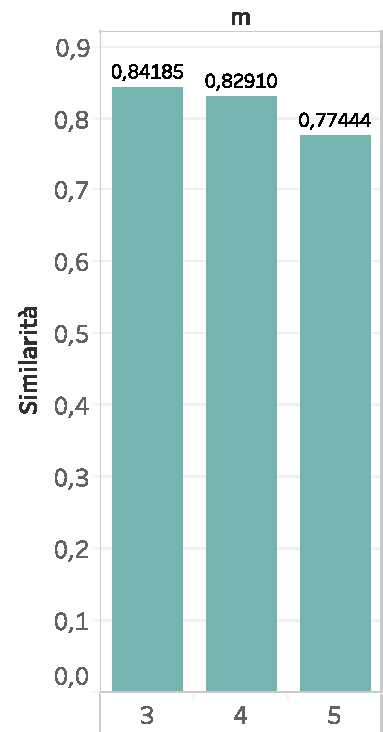
\includegraphics[scale=0.6]{res/fig/sec-4/scalability/ComparisonMSimilarity.pdf}
  \caption{Similarità \(S_{minus}\)}%
\end{subfigure}%
\begin{subfigure}{.5\textwidth}
  \centering
   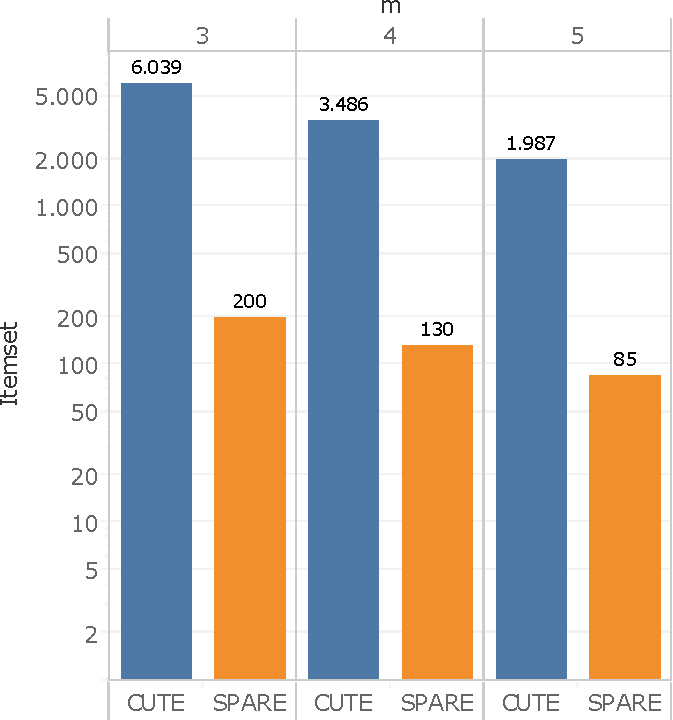
\includegraphics[scale=0.6]{res/fig/sec-4/scalability/ComparisonMCUTESPARE.pdf}
  \caption{Itemset individuati su CUTE e SPARE}%
  \end{subfigure}%
  \caption{Similarità a sinistra, itemset a destra al variare della dimensione minima dei gruppi \(m\)}%
  \label{fig:chap-4:CompM}
\end{figure}

\begin{figure}
  \centering
   \begin{subfigure}{.5\textwidth}
  \centering
      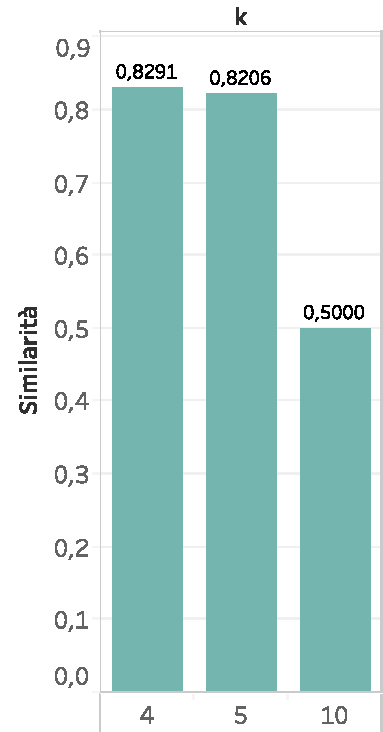
\includegraphics[scale=0.6]{res/fig/sec-4/scalability/ComparisonKSimilarity.pdf}
  \caption{Similarità \(S_{minus}\)}%
\end{subfigure}%
\begin{subfigure}{.5\textwidth}
  \centering
   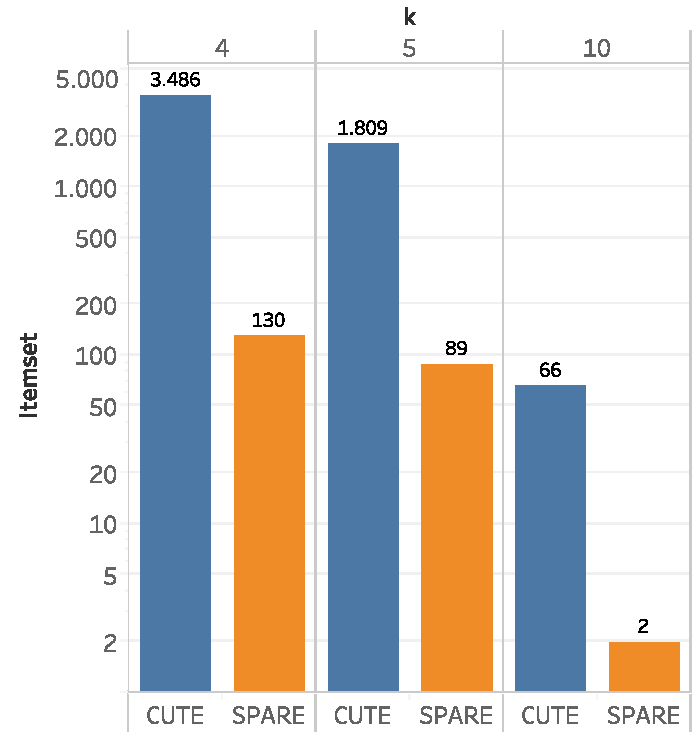
\includegraphics[scale=0.6]{res/fig/sec-4/scalability/ComparisonKCUTESPARE.pdf}
  \caption{Itemset individuati su CUTE e SPARE}%
  \end{subfigure}%
  \caption{Similarità a sinistra, itemset a destra al variare del supporto minimo \(k\)}%
  \label{fig:chap-4:CompK}
\end{figure}


Al variare di \(m\) (\cref{fig:chap-4:CompM}), è possibile vedere come all'aumentare delle dimensioni dei gruppi, la similarità totale tenda a calare.
Discorso analogo vale per \(k\): al suo aumentare la similarità totale cala.
Questo può essere giustificato sulla base delle divergenze nel determinare la vicinanza spaziale tra i due algoritmi.
Impostando infatti vincoli più rigidi, verranno riconosciuti itemset con maggiori dimensioni e supporto.
All'aumento di queste due misure corrisponde un incremento della possibilità che la composizione dei gruppi individuati tra i due algoritmi cambi.

Trattando invece di \(g\) \cref{fig:chap-4:CompG}, al rilassamento della continuità aumenta la similarità.
Anche questo è collegato con quanto detto sopra: pattern swarm contenenti gli stessi oggetti possono essere individuati in situazioni differenti.
È più raro che ciò possa accadere invece con pattern continui nel tempo, come ad esempio flock.

\begin{figure}
  \centering
   \begin{subfigure}{.5\textwidth}
  \centering
      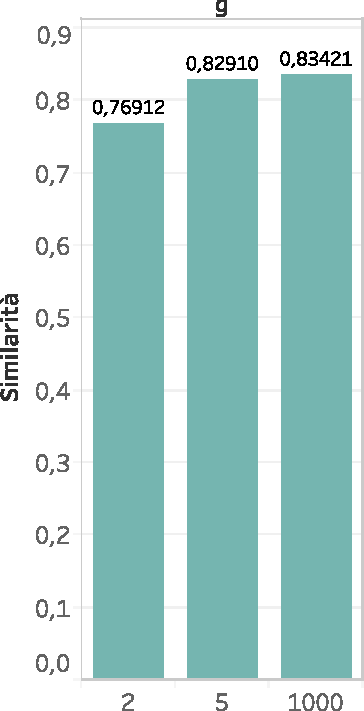
\includegraphics[scale=0.6]{res/fig/sec-4/scalability/ComparisonGSimilarity.pdf}
  \caption{Similarità \(S_{minus}\)}%
\end{subfigure}%
\begin{subfigure}{.5\textwidth}
  \centering
   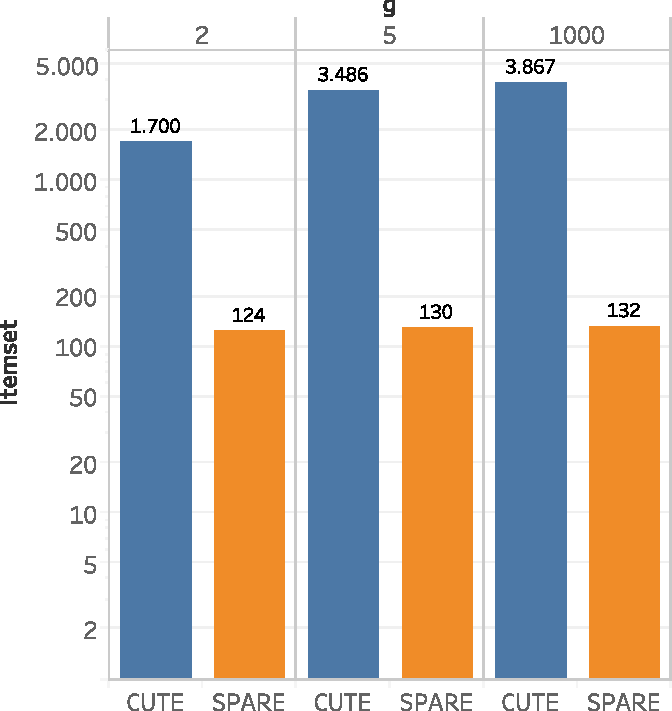
\includegraphics[scale=0.6]{res/fig/sec-4/scalability/ComparisonGCUTESPARE.pdf}
  \caption{Itemset individuati su CUTE e SPARE}%
  \end{subfigure}%
  \caption{Similarità a sinistra, itemset a destra al variare della continuità sul tempo \(g\)}%
  \label{fig:chap-4:CompG}
\end{figure}

Infine al variare di \(s\) si può vedere come il valore di similarità migliore si ottenga con il valore medio di \(s\).
La spiegazione di ciò può essere ricondotta alla distribuzione dei dati nello spazio.
Purtroppo è difficile determinare con precisione il valore ottimale di \(s\), se non determinandolo sperimentalmente.
Nonostante questo, \(1.75\) risulta un buon valore: quasi il \(50\%\) degli itemset di SPARE sono coperti da CUTE e la similarità complessiva è dell'\(80\%\). 

\begin{figure}
  \centering
   \begin{subfigure}{.5\textwidth}
  \centering
      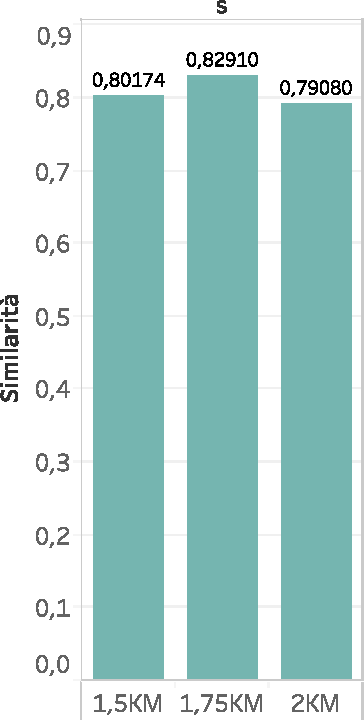
\includegraphics[scale=0.6]{res/fig/sec-4/scalability/ComparisonSSimilarity.pdf}
  \caption{Similarità \(S_{minus}\)}%
\end{subfigure}%
\begin{subfigure}{.5\textwidth}
  \centering
   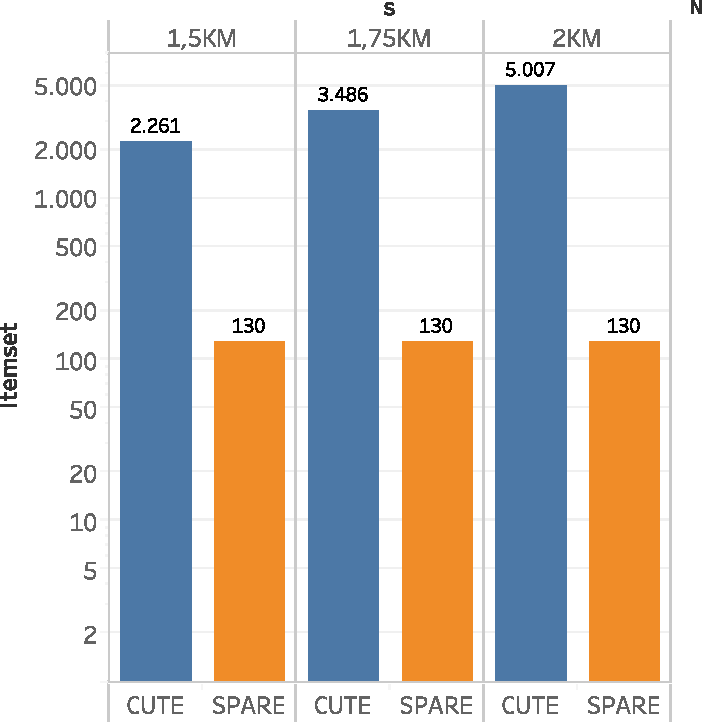
\includegraphics[scale=0.6]{res/fig/sec-4/scalability/ComparisonSCUTESPARE.pdf}
  \caption{Itemset individuati su CUTE e SPARE}%
  \end{subfigure}%
  \caption{Similarità a sinistra, itemset a destra al variare dell'area spaziale coperta dalle celle \(s\)}%
  \label{fig:chap-4:CompS}
\end{figure}


\subsection{Interpretazione dei risultati}\label{subsec:comp:result-evaluation}
Anche utilizzando definizioni di similarità personalizzate sul problema, i risultati fra i due cluster sono comunque molto diversi fra di loro.

Sicuramente entrambi gli algoritmi formalizzano la ricerca di pattern di co-movimento con alcuni elementi in comune, tuttavia l'approccio alla ricerca e la natura stessa degli itemset individuati porta a escludere una casistica reale in cui gli algoritmi individuano esattamente gli stessi cluster.
È però possibile tentare di massimizzare l'intersezione tra i risultati di questi due algoritmi, sempre tenendo presente che le cardinalità di CUTE sono di molto superiori a quelle di SPARE.

In teoria a parità di risultati sul clustering spaziale dovrebbe garantire quanto meno la totale sovrapposizione totale dei risultati di SPARE su quelli di CUTE.
Questo perché il tempo viene processato nello stesso modo dai due algoritmi, mentre invece lo spazio no.
Tuttavia trovare questo punto di intersezione è praticamente impossibile, SPARE valuta i cluster ad ogni istante temporale, definendo potenzialmente una configurazione spaziale diversa ad ogni istante.
La divisione effettuata da CUTE invece è fissa in tutti gli istanti temporali.

Sia CUTE che SPARE dispongono poi di vincoli che l'altro non non è in grado di coprire.
Questi devono essere necessariamente rilassati durante il confronto, per non far divergere ulteriormente i risultati.
Ciò però implica che il potenziale espressivo di questi parametri sia perso nella ricerca.

In definitiva CUTE e SPARE pongono due approcci che possono convergere parzialmente nella ricerca di pattern di co-movimento.
Allo stesso tempo tuttavia portano un contributo unico alla ricerca che viene minimizzato quando si vuole far convergere i risultati.





%---------------- TIME TEST











%------------- SCALABILITY TEST






%------- COMPARISON TEST



